\pagestyle{myFancy}
\chapter{Symmetries and Non-Hypercubic Lattices}

\section{Spacetime Symmetry Restoration}
The restoration of spacetime symmetries in the continuum limit is an important aspect of lattice field theory.
Minkowskian spacetime is invariant under the action of the Poincaré group, that includes translations, rotations in the $3$-dimensional space, and boosts.
When performing the Wick rotation, boosts become rotations in the planes formed by each spatial axis and the Euclidean time.
The Euclidean spacetime is therefore invariant, in the continuum, under translations:
\begin{equation}
    x^\mu \to x^\mu + \varepsilon^\mu \label{3:TranslCont}
\end{equation}
and under rotations in $4$ dimensions:
\begin{equation}
    x^\mu \to R^\mu_\nu x^\nu \qquad\text{with}\qquad R\in\Orot(4) \label{3:RotCont}
\end{equation}
These invariances do not hold anymore once the space is discretized: a generic lattice is, in fact, invariant only under translations by integer multiples of the elementary lattice vectors:
\begin{equation}
    x \to x + a\mu \qquad\text{with}\qquad x\in\Lambda \label{3:TraslDiscr}
\end{equation}
and under certain rotations:
\begin{equation}
    x \to \Gamma x \qquad\text{with}\qquad x\in\Lambda, \Gamma\in G_\Lambda \label{3:RotDiscr}
\end{equation}
where $G_\Lambda\subset\Orot(4)$ is a discrete subset of the full rotational group $\Orot(4)$ that depends on the lattice $\Lambda$.
For example, $\Lambda=\Lambda_{SH}$ is a SH lattice, then $G_{\Lambda_{SH}}$ is the $384$-elements group with all possible reflections on every coordinate plane and rotations of multiples of $90^\degree$ around each one of the $4$ axis.\\
The fact that the symmetries in the lattice theory and in the continuum theory are different is not a problem in itself, as long as when approaching the continuum limit the symmetries of the continuum theory are recovered.
This is the case for the translational symmetry: if $a\to0$, \eqref{3:TraslDiscr} becomes \eqref{3:TranslCont}.
However, the rotational symmetry is not restored (at least, not naively) when the continuum limit is taken: (\eqref{3:RotDiscr} does not become \eqref{3:RotCont} when $a\to0$), as the Simple Hypercubic lattice is invariant under rotations of multiples of $90^\degree$ independently from the value of the lattice spacing.\\
However, the restoration of continuum symmetries is more subtle than this intuition: in the lattice theory, it typically happens that the terms breaking the continuum rotational symmetry down to its discrete subgroup that is manifest on the lattice are actually suppressed by powers of the lattice spacing in the $a\to 0$ limit. This suppression, however, may fail, if the coefficients of the terms associated with higher powers of $a$ are, instead, divergent in the continuum limit. For this reason, studies on the restoration of rotational symmetry have been made, through the computation of quantities that are expected to exhibit rotational invariance in the continuum theory.

\subsection{Rotational Invariance of the Static Quark Potential\label{Sec3:RotInv}}
An example of these studies is provided by a 1982 article by Lang and Rebbi~\cite{Lang:1982tj}, where the static quark potential $V(r)$, obtained from the correlator of two Polyakov loops (see \eqref{1:PolyakovPotential}), was studied at different lattice spacings in the $\SU(2)$ lattice gauge theories. The potential
\begin{equation}
    V(r) = -T\ln\expval{P^\dagger(r)P(0)} \label{3:LangRebbiPotential}
\end{equation}
was obtained from simulations for different values of $r=(r_x, r_y, r_z)$ on lattices extending for $n_s$ lattice spacings in each of the space directions and $n_t$ lattice sites in the time direction.
In this work, the full gauge group $\SU(2)$ was actually approximated by its discrete icosahedral subgroup $\tilde{Y}$ (due to the computing power limitations of that time).
The various (about $1000$) potentials obtained for each site $r$ were then fitted according to the expected form for a linearly confining potential
\begin{equation}
    V(r) = c_0 + c_1/r + c_2r \label{3:LangRebbiPotentialFit}
\end{equation}
A representation of the equipotential surfaces of expression \eqref{3:LangRebbiPotentialFit} is reproduced in \figref{3F:LangRebbi}.
\begin{figure}[!htbp]
    \centering
    \hfill
    \begin{subfigure}[b]{0.45\textwidth}
        \centering
        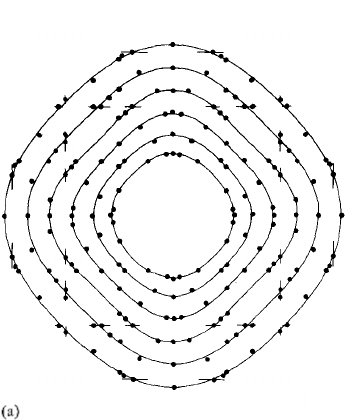
\includegraphics[width=0.857\textwidth]{LangRebbi_a.png}
        \caption{$\beta=2$, $n_s=8$, $n_t=4$.}
        \label{3F:LangRebbiA}
    \end{subfigure}
    \begin{subfigure}[b]{0.45\textwidth}
        \centering
        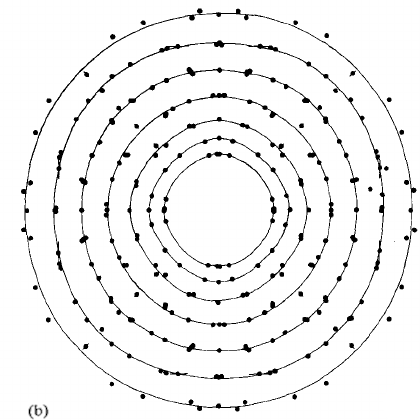
\includegraphics[width=\textwidth]{LangRebbi_b.png}
        \caption{$\beta=2.25$, $n_s=16$, $n_t=6$.}
        \label{3F:LangRebbiB}
    \end{subfigure}
    \hfill
    \caption{Representation of equipotential surfaces for larger (\ref{3F:LangRebbiA}) and smaller (\ref{3F:LangRebbiB}) lattice spacing.}
    \label{3F:LangRebbi}
\end{figure}\\
In \figref{3F:LangRebbiA} a lattice with $n_s=8$, $n_t=4$ and $\beta=\frac4{g^2}=2$ was used, while \figref{3F:LangRebbiB} was obtained from data obtained on a lattice with $n_s=16$, $n_t=6$ and $\beta=2.25$.
Given that, at the leading order in perturbation theory, the lattice spacing depends on $\beta$ in the following way:
\begin{equation}
    a(\beta) \approx e^{-\frac{12\pi^2}{11N^2}\beta} = e^{-\frac{3\pi^2}{11}\beta} \label{3:BetaLatticeSpacing} 
\end{equation}
the first plot corresponds to a higher value of $a$ than the second one\footnote{The rigorous determination of the lattice spacing is a rather compliacted matter that will not be explained further, as it is not the purpose of this project.}.\\
As can be easily seen, by lowering the lattice spacing equipotential surfaces tend to become circles, therefore the rotational invariance, that is broken in the lattice for any value of the lattice spacing, gets restored in the expectation value of the observables, making lattice field theory a \emph{``good''} theory capable of making meaningful predictions.

\section{Other Types of Lattice\label{Sec3:Lattices}}
In \secref{Sec1:SHLattice} the Simple Hypercubic lattice has been defined.
Of course, it is not the only possible choice, although it is the simplest.
In fact, in order to further investigate the restoration of rotational symmetry and to make better predictions on rotational invariant quantities, other types of lattices have been used to simulate lattice field theories.

\subsection{Body-Centered Tesseract\label{Sec3:BCT}}
For example, the Body-Centered Tesseract (BCT) has been used for simulation of Yang-Mills theories.
It consists of packing the spacetime with tesseracts, as the name suggests, but considering both the corners and the centers of every hypercube as lattice sites (see \figref{3F:ScBccCells} for a tridimensional representation of a cubic cell \eqref{3F:CubicCell} and a body-centered cubic cell \eqref{3F:BCCubicCell}).\\
\begin{figure}[!htbp]
    \centering
    \hspace{0.1\textwidth}
    \begin{subfigure}[b]{0.25\textwidth}
        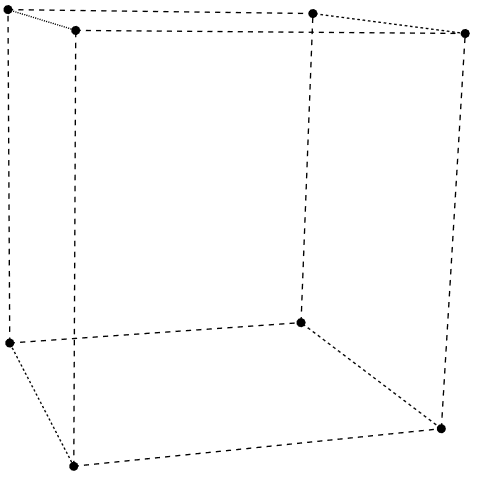
\includegraphics[width=\textwidth]{CubicCell.png}
        \caption{Simple cube.}
        \label{3F:CubicCell}
    \end{subfigure}
    \hspace{0.2\textwidth}
    \begin{subfigure}[b]{0.25\textwidth}
        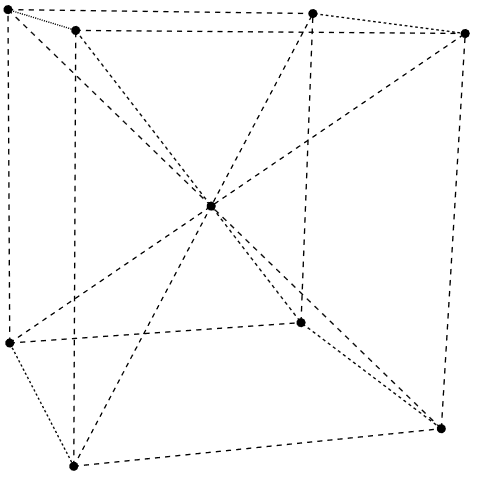
\includegraphics[width=\textwidth]{BodyCenteredCubicCell.png}
        \caption{Body-centered cube.}
        \label{3F:BCCubicCell}
    \end{subfigure}
    \hspace{0.2\textwidth}
    \caption{Tridimensional representation of a simple cubic cell (\ref{3F:CubicCell}) and a body-centered one (\ref{3F:BCCubicCell}).}
    \label{3F:ScBccCells}
\end{figure}\\
Every site of the BCT lattice has, therefore, $24$ nearest neighbours: $16$ are identified by all possible sign permutations of $\pr{\pm\frac12,\pm\frac12,\pm\frac12,\pm\frac12}$, the $8$ remaining are the ones of the SH lattice.
The cell of this lattice is known as $24$-cell, shown in \figref{3F:24cell}, and the plaquettes are triangular.
\begin{figure}[!htbp]
    \centering
    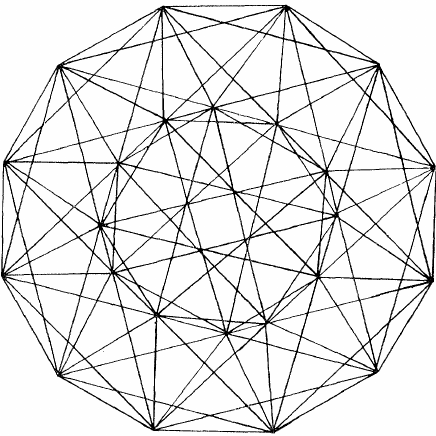
\includegraphics[width=0.33\textwidth]{24cell.png}
    \caption{Bidimensional projection of the $24$-cell.}
    \label{3F:24cell}
\end{figure}\\
This lattice has a $1152$-elements symmetry group $G_{\Lambda_{BCT}}$, i.e., significantly more rotations and reflections than the $384$ of the SH lattice.

\subsection{\spFtext Coroots Lattice}
\spFtext is one of the five exceptional simple Lie groups, with Dynkin diagram \dynkin F4.
A more detailed explanation of exceptional Lie groups and algebras can be found in~\cite{adams1996lectures}.
Its root lattice is a $4$-dimensional body-centered hypercubic lattice, a BCT, while its dual, that is called the \spFtext coroots lattice, is the $4$-dimensional lattice with the symmetry group of highest order.
Each site of this lattice has $48$ nearest neighbours:
\begin{itemize}
    \item $24$ corresponding to the roots of \spFtext, individuated by all possible sign and position permutations of $(\pm1,\pm1,0,0)$;\
    \item $24$ corresponding to the coroots, the roots' dual vectors, individuated by\
    \begin{itemize}
        \item[$\circ$] the $8$ possible sign and coordinate permutations of $(\pm1,0,0,0)$\
        \item[$\circ$] the $16$ possible sign permutations of $\pr{\pm\frac12,\pm\frac12,\pm\frac12,\pm\frac12}$\
    \end{itemize}
\end{itemize}
This lattice is made up of two BCT lattices: the first one is the dual lattice, that is the same as \secref{Sec3:BCT}, the other is the root lattice, that is a BCT with lattice spacing $\sqrt2$ as can be seen as represented in \figref{3:F4cell}.
\begin{figure}[!htbp]
    \centering
    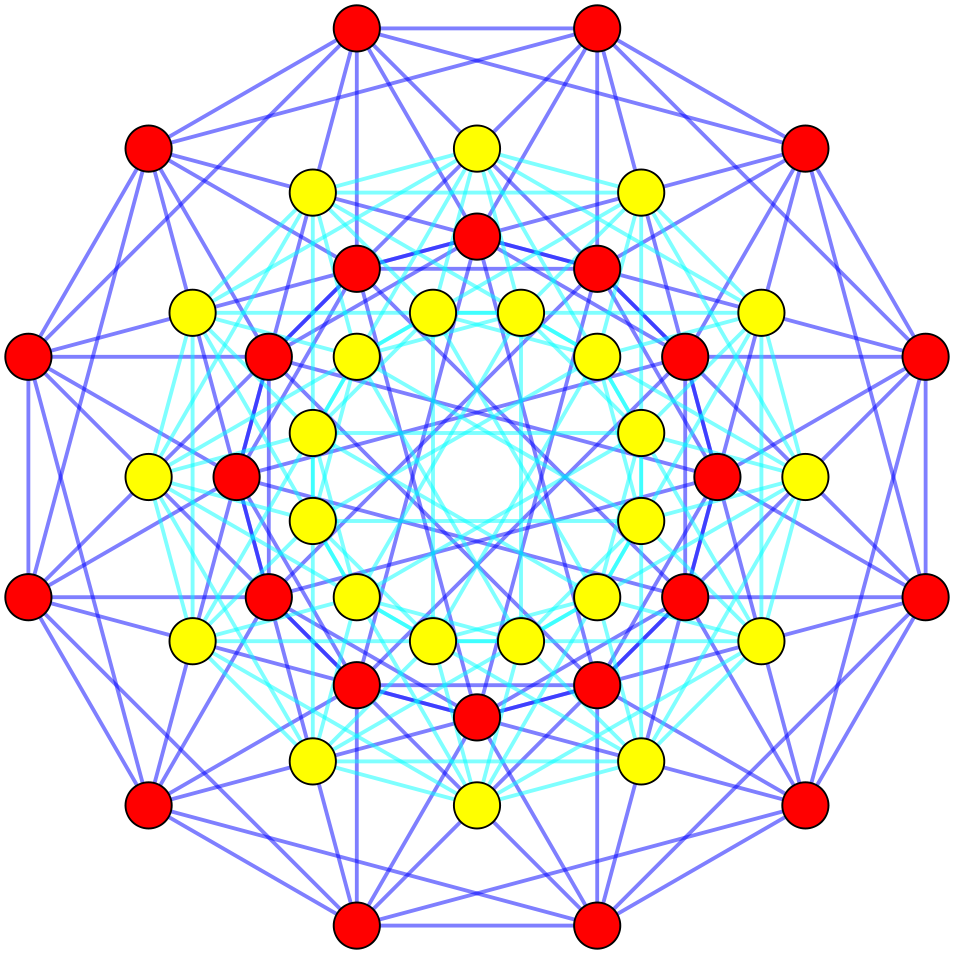
\includegraphics[width=0.33\textwidth]{F4_root_lattice.png}
    \caption{Bidimensional projection of the elementary cell of the \spFtext coroots lattice.\\
             The roots are represented in red and the coroots in yellow.}
    \label{3:F4cell}
\end{figure}\\
This lattice has a symmetry group $G_{\Lambda_{\spF}}$ of order $2304$, twice as the BCT symmetry group.

\section{Simulations on Higher Symmetric Lattices}
These lattices have been used, in literature, to perform Monte Carlo simulations of quantum field theories.

\subsection{Scalar Fields on \spFtext Lattice}
In~\cite{Neuberger:1987kt}, Neuberger presented the formulation of scalar fields in terms of the \spFtext lattice, where he discretized the action \eqref{1:ScalarActionEuclidean} assuming the simplest nearest neighbours interaction:
\begin{equation}
    S = \frac16\sum_{<xy>\in\Lambda}\pr{\phi(x)-\phi(y)}^2 +\sum_{x\in\Lambda}\pr{\frac12m^2\phi^2(x)+\frac\lambda4\phi^4(x)} \label{3:ScalarActionF4}
\end{equation}
where $<xy>$ indicates sum over nearest neighbours.\\
The Fourier transform of the field $\phi(x)$ in the limit of infinite lattice volume is given by:
\begin{align*}
    \tilde\phi(k) =& \dV e^{\i k \cdot x} \phi(x) \\
    \phi(x) =& \frac1{2(2\pi)^4} \int\dd^4k e^{-\i k \cdot x} \tilde\phi(k)
\end{align*}
and the kinetic energy of \eqref{3:ScalarActionF4} at infinite volume is:
\begin{align*}
    \text{K.E.} =& \frac1{6(2\pi)^4} \int\dd^4k \abs{\tilde\phi(k)}^2\pr{\sum_\mu\pr{1-\cos(k_\mu)} +\sum_\pm\pr{1-\cos(\frac{k_1\pm k_2\pm k_3\pm k_4}{2})}} =\\
    =& \frac{1}{12(2\pi)^4} \int\dd^4k \abs{\tilde\phi(k)}^2\pr{k^2-\frac{1}{72}k^4+O(k^6)} \numthis\label{3:ScalarKE}
\end{align*}
The fact that the fourth-order term is proportional to the square of the second-order one is a signature of the symmetry-preserving nature of this lattice action.\\
This work lead to some analytical~\cite{Bhanot:1990zd} and numerical~\cite{Bhanot:1990ai} results and to an upper bound prediction on the mass of the Higgs boson~\cite{Heller:1990sg} more than $20$ years before its actual discovery.

\subsection{Gauge Theories on the BCT Lattice\label{Sec3:BCTlatticeGaugeTheories}}
In~\cite{Celmaster:1982ht}, Celmaster presented the first computations for an $\SU(2)$ theory on a BCT.
Being a different lattice, where the plaquette is a triangle and not a square, a new action has to be defined. An action that is invariant under the BCT group, with the correct classical continuum limit is:
\begin{equation}
    S_{BCT} = \frac1{2g^2} \sum_\bigtriangleup \Re\Tr \Utriang = \frac\beta8 \sum_\bigtriangleup \Re\Tr \Utriang \label{3:BCTAction}
\end{equation}
where $\Utriang$ is the triangular plaquette, defined as
\begin{equation}
    \Utriang = U_v(x)U_w(x+\hat{v})U_{-v-w}(x+\hat{v}+\hat{w}) = U_v(x)U_w(x+\hat{v})U^\dagger_{v+w}(x) \label{3:PlaqTriang}
\end{equation}
where $v$ and $w$ are labels indicating the possible nearest-neighbour directions, described in \secref{Sec3:BCT}, such that $v+w$ is a valid direction.
\begin{comment}
\begin{figure}[!hbtp]
    \centering
    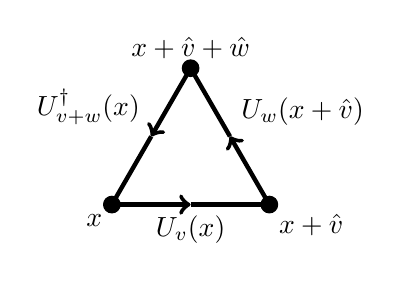
\begin{tikzpicture}
        \filldraw[black]  (0,0) circle (3pt) node[anchor=north east]{$x$};
        \filldraw[black]  (2,0) circle (3pt) node[anchor=north west]{$x+\hat{v}$};
        \filldraw[black]  (1,1.732) circle (3pt) node[anchor=south]{$x+\hat{v}+\hat{w}$};
        \draw[ultra thick,->] (0,0) -- (1,0) node[anchor=north]{$U_v(x)$};
        \draw[ultra thick   ] (1,0) -- (2,0);
        \draw[ultra thick,->] (2,0) -- (1.5,0.866) node[anchor=south west]{$U_w(x+\hat{v})$};
        \draw[ultra thick   ] (1.5,0.866) -- (1,1.732);
        \draw[ultra thick,->] (1,1.732) -- (0.5,0.866) node[anchor=south east]{$U^\dagger_{v+w}(x)$};
        \draw[ultra thick   ] (0.5,0.866) -- (0,0);
    \end{tikzpicture}
    \caption{Schematization of an elementary triangular plaquette.}
    \label{3F:PlaqTriang}
\end{figure}\\
\end{comment}
\begin{figure}[!hbtp]
    \centering
    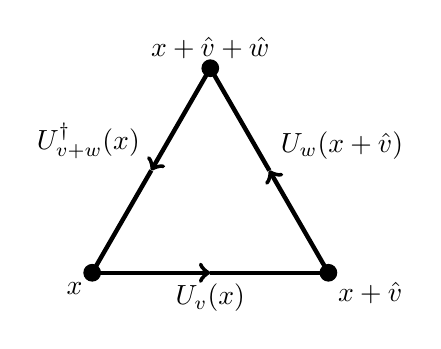
\begin{tikzpicture}
        \filldraw[black]  (0,0) circle (3pt) node[anchor=north east]{$x$};
        \filldraw[black]  (3,0) circle (3pt) node[anchor=north west]{$x+\hat{v}$};
        \filldraw[black]  (1.5,2.598) circle (3pt) node[anchor=south]{$x+\hat{v}+\hat{w}$};
        \draw[ultra thick,->] (0,0) -- (1.5,0) node[anchor=north]{$U_v(x)$};
        \draw[ultra thick   ] (1.5,0) -- (3,0);
        \draw[ultra thick,->] (3,0) -- (2.25,1.299) node[anchor=south west]{$U_w(x+\hat{v})$};
        \draw[ultra thick   ] (2.25,1.299) -- (1.5,2.598);
        \draw[ultra thick,->] (1.5,2.598) -- (0.75,1.299) node[anchor=south east]{$U^\dagger_{v+w}(x)$};
        \draw[ultra thick   ] (0.75,1.299) -- (0,0);
    \end{tikzpicture}
    \caption{Schematization of an elementary triangular plaquette.}
    \label{3F:PlaqTriang}
\end{figure}\\
For example, if $v=(+1,0,0,0)$ and $w=(0,+1,0,0)$, then they add up to $v+w=(+1,+1,0,0)$, that is not one of the nearest-neighbours vectors, whereas $v=(+1,0,0,0)$ and $w=\pr{-\frac12,+\frac12,-\frac12,+\frac12}$ add up to $v+w=\pr{+\frac12,+\frac12,-\frac12,+\frac12}$, that is a valid direction.
In \figref{3F:PlaqTriang}, an example of an elementary triangular plaquette is shown.\\
There are $96$ such triangles touching each site, and each edge is shared by $8$ triangles.
By comparison, on the SH lattice there are $24$ elementary square plaquettes touching each site and each edge is contiguous to $6$ squares.\\
In~\cite{Celmaster:1983hs} and~\cite{Celmaster:1983vy} Celmaster presented the first simulation results for the $\SU(2)$ gauge theory on the BCT lattice, explaining the algorithm used for the simulations in \cite{CELMASTER1985415}.

\subsubsection{Average Plaquette Value on BCT}
In~\cite{Celmaster:1983vy} a study on the average value of the plaquette was presented: it is plotted \wrt $\beta$ in \figref{3F:AvgPlaqBCTSH}.\\
As can be seen, the BCT average plaquette better follows the strong and weak coupling expansions, that are analytical approximations valid, respectively, for $\beta\to0$ ($\Leftrightarrow g\to\infty$) and for $\beta\to\infty$ ($\Leftrightarrow g\to0$).
\begin{figure}[!htbp]
    \centering
    \begin{subfigure}[b]{0.475\textwidth}
        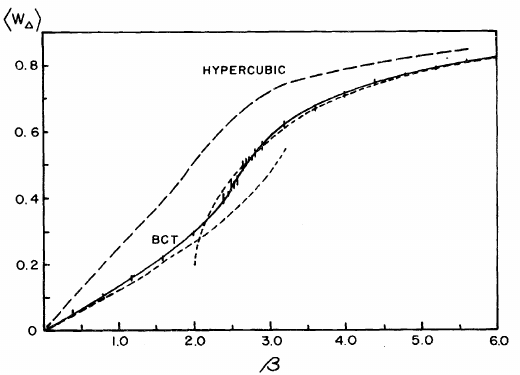
\includegraphics[width=\textwidth]{AvgPlaq1.png}
        \caption{Comparison between $\expval{W_\bigtriangleup}$ on BCT and SH lattices. The short-dashed lines represent weak and strong coupling expansions.}
        \label{3F:AvgPlaqBCTSH}
    \end{subfigure}
    \hfill
    \begin{subfigure}[b]{0.475\textwidth}
        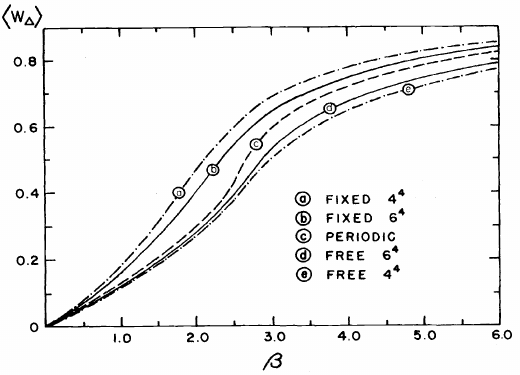
\includegraphics[width=\textwidth]{AvgPlaq2.png}
        \caption{Dependence of $\expval{W_\bigtriangleup}$ on boundary conditions in different BCT lattices, with different boundary conditions.}
        \label{3F:AvgPlaqBoundary}
    \end{subfigure}
    \caption{Average value of the plaquette $\expval{W_\bigtriangleup}$ on a BCT lattice as a function of $\beta$.}
\end{figure}\\
In the same article the influence of the boundary conditions on the average value of the plaquette was also investigated.
Three different types of boundary conditions were considered: periodic, that means that lattice has the topology of a $4$-dimensional torus, free, that means that links on the boundary are free to take any $\SU(2)$ value, and fixed, that means that links on the boundary are constrained to take a certain $\SU(2)$ value.
The results are plotted in \figref{3F:AvgPlaqBoundary}.\\
From the plot, it can be seen that $\expval{W_\bigtriangleup}_{free} \leq \expval{W_\bigtriangleup}_{periodic} \leq \expval{W_\bigtriangleup}_{fixed}$, which is an inequality discussed by Mütter and Schilling in~\cite{Konig:1983dg}.\\
It was also pointed out that the computing time of BCT simulations was larger by a factor of approximately $2.5$ as compared with SH simulations: this is due to having $3$ times as many degrees of freedom, that become $\frac{11}{3}$ as many if a gauge fixing is done, and $\frac{16}{3}$ as many plaquettes for each site.
However, having $12$ symmetry axes instead of $4$ provides a higher symmetry of the observables allowing for better checks on computations.

\subsubsection{String Tension}
In~\cite{Celmaster:1983hs} the $\SU(2)$ string tension was obtained from measurements of ratios of Wilson loops on a $6^4$ BCT lattice.\\
On a BCT lattice, there are two types of Wilson loops:
\begin{itemize}
    \item Rectangular Wilson loops $W_R(n,m)=\frac12\expval{\Tr U_R(n,m)}$\
    \item Triangular Wilson loops $W_T(n)=\frac12\expval{\Tr U_T(n)}$
\end{itemize}
where $U_R(n,m)$ is the product of link variables over an $n\times m$ rectangle and $U_T(n)$ is the product of link variables over an equilateral triangle of side $n$.\\
Assuming that Wilson loops are fitted by:
\begin{equation}
    W = e^{-\sigma A -b(\text{perimeter}) +\text{const.}} \label{3:WilsonFit}
\end{equation}
where $A$ is the area of the loop, then the string tension $\sigma$ can be obtained through logarithmic ratios (also called \emph{Creutz ratios}):
\begin{align}
    \chi(2) =& -\ln(\frac{W_R(1,1)W_R(2,2)}{W_R^2(1,2)}) \\
    R_T(3) =& -\frac{2}{\sqrt3}\ln(\frac{W_T(1)W_T(3)}{W_T^2(2)})
\end{align}
Results of the simulations are plotted in \figref{3F:LogLoopRatios}, assuming no correlations between loop fluctuations in the computation of the error bars.
\begin{figure}[!htbp]
    \centering
    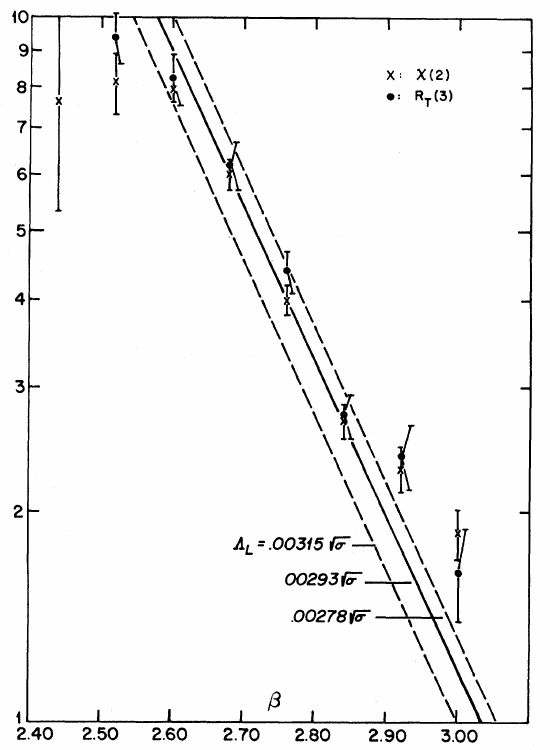
\includegraphics[width=0.4\textwidth]{LogarithmicRatios.png}
    \caption{$\SU(2)$ logarithmic loop ratios as a function of $\beta$ on a $6^4$ BCT lattice.}
    \label{3F:LogLoopRatios}
\end{figure}\\
The logarithmic loop ratio $\chi(2)$ agrees with the asymptotic freedom curve in the region $2.68\leq\beta\leq2.84$ far better than any other result obtained with simulations on SH lattices.
This is a consequence of the fact that the BCT action has smaller $O(a^2)$ corrections than usual at small $\beta$, therefore finite-spacing corrections are smaller for this action than for the action on a SH lattice.
Therefore, BCT lattices with less sites than SH lattices could be used to obtain data with the same accuracy, at a given physical hypervolume.\\
%In the article it was pointed out that, if the lattice spacing is sent $a\to a/2$, a SH lattice would require $16$ times as many sites in order to keep the physical size of the Wilson loop constant, while if the same operation is done on a BCT lattice, the increment in the number of sites would be much less, using about $16$ times less CPU time than the Wilson action.\\
Furthermore, $R_T(3)$ is compatible with $\chi(2)$ within the statistical uncertainties: this is a confirmation of the area-law dependence of equation \eqref{3:WilsonFit}.\\
In conclusion, simulations on BCT lattices provide better results, with more rotational invariance than those on other lattices, at a cost of a (slightly) higher computational time.
